\documentclass{article}
\usepackage{tikz}
\usetikzlibrary{positioning}

\begin{document}

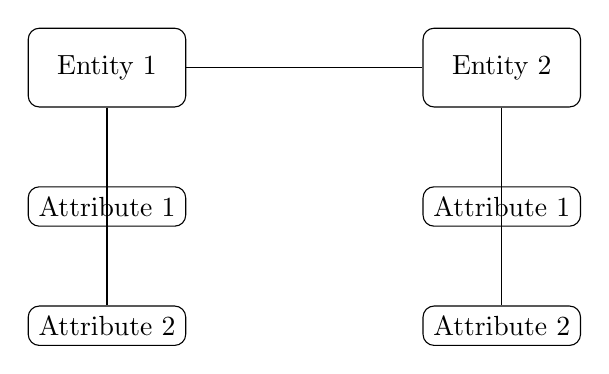
\begin{tikzpicture}[entity/.style={draw, rectangle, rounded corners, minimum width=2cm, minimum height=1cm, align=center},
    attribute/.style={draw, rectangle, rounded corners, minimum width=2cm, minimum height=0.5cm, align=center}]

% Define the entities and their attributes
\node[entity] (E1) {Entity 1};
\node[attribute, below=of E1] (A1) {Attribute 1};
\node[attribute, below=of A1] (A2) {Attribute 2};

% Draw lines connecting the entity to its attributes
\draw (E1) -- (A1);
\draw (E1) -- (A2);

% Define another entity and its attributes
\node[entity, right=3cm of E1] (E2) {Entity 2};
\node[attribute, below=of E2] (B1) {Attribute 1};
\node[attribute, below=of B1] (B2) {Attribute 2};

% Draw lines connecting the second entity to its attributes
\draw (E2) -- (B1);
\draw (E2) -- (B2);

% Optionally, draw a line connecting the two entities if they are related
\draw (E1) -- (E2);

\end{tikzpicture}

\end{document}